% \documentclass{report}
% 
% \usepackage{fancyhdr}
\usepackage{fourier-orns}
\usepackage{hyperref}%% To refrence links / jumps
\usepackage{chngcntr} %% For some extra counters numberings
\usepackage[a4paper, right = 0.5in, left = 0.5in,top = 1in , bottom = 1in]{geometry}
\usepackage{etoolbox} %% Provides like a language for advanced customization
\usepackage{datetime} %% For dates of course
\usepackage{lastpage} %% provides pages numbers
\usepackage[sc]{titlesec} %% modify titles
\usepackage{enumerate}
\usepackage{cancel}
\usepackage{tikzsymbols}
\usepackage[dvipsnames]{xcolor}
\usepackage{import}
\usepackage{pdfpages} %% include other pdfs
\usepackage{transparent} %% Transparency
\usepackage{xcolor}  %% Colors
\usepackage[many]{tcolorbox}
\usepackage[framemethod=TikZ]{mdframed}
\usepackage{amsmath,amsfonts,amsthm,amssymb,mathtools}
\usepackage{tikz}
\usepackage{bookmark}
\usepackage{graphicx}
\usepackage{mathpazo}

\usepackage{fontawesome5}

\linespread{1.5}


\titleformat{\chapter}[display]   
{\fontfamily{ppl}\selectfont\huge\color{YellowOrange!80!orange}} % Font style and size 
{\raggedleft\color{purple}\fontsize{70}{0pt}\selectfont\thechapter}   
{-1.5cm}    			                          % Space between the chapter number and title
{
	\begin{tikzpicture}[overlay]
		\node[anchor = west,yshift = 0.2cm,xshift = -1cm] {\fontsize{90}{20} $\int_{}^{} $};
		\node[yshift = 4cm, xshift = 17cm]   {\includegraphics[width = 4cm]{preview0}};
	\end{tikzpicture}
\hspace{1cm}\Huge\raggedright\MakeUppercase}

\titleformat{\section}[block]
{
\fontfamily{ppl}\selectfont\huge\color{YellowOrange!80!orange}
}
{
\color{purple}\fontsize{20}{0pt}\selectfont\thesection 
}
{0cm}
{
	\begin{tikzpicture}[overlay]
		\node[anchor = west,yshift = 0.2cm,xshift = -0.4cm, circle = 1pt] {};
	\end{tikzpicture}
}

\titlespacing*{\section}{0pt}{0.7cm}{1.5cm}


\newcommand{\divider}
{
	\begin{center}
	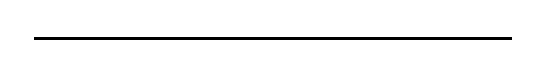
\begin{tikzpicture}
		\draw[thick, black] (0.25*\textwidth, 0) -- (0.75*\textwidth, 0);
		\node[rotate = 360 - 90, xshift = -0.6pt, yshift = 1pt] at (0.25*\textwidth,0){\decotwo};
		\node[rotate = 90, xshift = -0.6pt, yshift = 1pt] at (0.75*\textwidth,0){\decotwo};
	\end{tikzpicture}
	\end{center}
}

\pagestyle{fancy}

\newcommand{\lecday}[1][]
{
    \def\datee{#1}
    \fancyhead[L]{\datee}
}



\newcommand{\signature}
{
	\begin{tikzpicture}[remember picture,overlay]
		\node[fill = YellowOrange!20!white] at ([yshift = 1cm, xshift = -3cm]current page.south east) {\fontsize{10pt}{0pt}{\itshape Kara.$\mathcal{A}$}};
	\end{tikzpicture}
}

\AddToHook{shipout/background}{
  \begin{tikzpicture}[remember picture, overlay]
	  \node[] at ([yshift = 1.5cm,xshift = \textwidth /2 + 0.9cm]current page.south west) {\includegraphics[width = 0.5cm]{preview3}};
	  \node[] at ([yshift = 1.5cm,xshift = - \textwidth /2 - 0.9cm]current page.south east) {\includegraphics[width = 0.5cm]{preview4}};
  \end{tikzpicture}
}



\newtcolorbox[auto counter, number within = section]{remark}[1][]
{
       		title = Remark #1,
		enhanced,
		boxrule = 0pt,
		colback = white,
		breakable,
		arc = 4pt,
		colbacktitle = cyan,
		colback = cyan!5!white,
		segmentation style =
		{
			solid,cyan,thick,
		},
		attach boxed title to top left =
		{
			xshift = 0cm,
		},
		boxed title style =
		{
			boxrule = 0pt,
			sharp corners,
			drop fuzzy shadow = {cyan},
		},
		drop fuzzy shadow = {cyan!80!black},
}

\newtcolorbox[auto counter, number within = section]{theorem}[1][]
{                                      
		title = Theorem \thetcbcounter : #1,
		enhanced, 
		boxrule = 0pt,
		colback = white,
		breakable,
		arc = 4pt,
		colbacktitle = purple,
		colback = purple!5!white,
		segmentation style = 
		{
			solid, purple,thick,
		},
		attach boxed title to top left = 
		{
			xshift = 0cm, 
		},
		boxed title style = 
		{
			boxrule = 0pt,
			sharp corners,
			drop fuzzy shadow = {purple},
		},
		drop fuzzy shadow = {purple!80!black},
}

\newtcolorbox[auto counter, number within = section]{definition}[1][]
{                                      
		title = Definition \thetcbcounter : #1,
		enhanced, 
		boxrule = 0pt,
		colback = white,
		arc = 4pt,
		breakable,
		colbacktitle = YellowOrange!80!black,
		segmentation style = 
		{
			solid, YellowOrange,thick,
		},
		attach boxed title to top left = 
		{
			xshift = 0cm, 
		},
		colback = YellowOrange!5!white,
		boxed title style = 
		{
			boxrule = 0pt,
			sharp corners,
			drop fuzzy shadow = {YellowOrange!80!orange},
		},
		drop fuzzy shadow = {YellowOrange!80!black},
}

\newtcolorbox[auto counter, number within = section]{corollary}[1][]
{                                      
		title = corollary \thetcbcounter : #1,
		enhanced, 
		boxrule = 0pt,
		colback = white,
		arc = 4pt,
		breakable,
		colbacktitle = YellowOrange!80!black,
		segmentation style = 
		{
			solid, YellowOrange,thick,
		},
		attach boxed title to top left = 
		{
			xshift = 0cm, 
		},
		colback = YellowOrange!5!white,
		boxed title style = 
		{
			boxrule = 0pt,
			sharp corners,
			drop fuzzy shadow = {YellowOrange!80!orange},
		},
		drop fuzzy shadow = {YellowOrange!80!black},
}


\newtcolorbox{example}[1][]
{                                      
		title = Example,
		enhanced, 
		boxrule = 0pt,
		colback = white,
		arc = 4pt,
		segmentation style = 
		{
			solid, SpringGreen,thick,
		},
		breakable,
		colback = SpringGreen!5!white,
		colbacktitle = SpringGreen!80!black,
		attach boxed title to top left = 
		{
			xshift = 0cm, 
		},
		boxed title style = 
		{
			boxrule = 0pt,
			sharp corners,
			drop fuzzy shadow = {SpringGreen!80!orange},
		},
		drop fuzzy shadow = {SpringGreen!80!black},
}


\newcommand{\integral}[4]{\int\limits_{#1}^{#2} #4 d#3}
\newcommand{\limit}[3]{\lim\limits_{#1 \rightarrow #2} #3}
\newcommand{\strone}[2]{\left[ \begin{gathered}#1\\ #2\end{gathered} \right] }
\newcommand{\strtwo}[2]{\left\{ \begin{gathered}#1\\ #2\end{gathered} \right\} }
\newcommand{\strthree}[2]{\left\lfloor \begin{gathered}#1\\ #2\end{gathered} \right\rfloor }


\newcommand{\startbf}[1]{\text{\bfseries{#1}}}
\newcommand{\sett}[1]{\left\{ #1 \right\}}
\newcommand{\thesis}[1]{\left( #1 \right)}
\newcommand{\brkt}[1]{\left[ #1 \right]}
\newcommand{\floor}[1]{\left\lfloor #1 \right\rfloor}


\DeclareMathOperator{\img}{im} % Image
\DeclareMathOperator{\Img}{Im} % Image
\DeclareMathOperator{\coker}{coker} % Cokernel
\DeclareMathOperator{\Coker}{Coker} % Cokernel
\DeclareMathOperator{\Ker}{Ker} % Kernel
\DeclareMathOperator{\rank}{rank}
\DeclareMathOperator{\Spec}{Spec} % spectrum
\DeclareMathOperator{\Tr}{Tr} % trace
\DeclareMathOperator{\pr}{pr} % projection
\DeclareMathOperator{\ext}{ext} % extension
\DeclareMathOperator{\pred}{pred} % predecessor
\DeclareMathOperator{\dom}{dom} % domain
\DeclareMathOperator{\ran}{ran} % range
\DeclareMathOperator{\Hom}{Hom} % homomorphism
\DeclareMathOperator{\Mor}{Mor} % morphisms
\DeclareMathOperator{\End}{End} % endomorphism


\newcommand{\lm}{\ensuremath{\lambda}}
\newcommand{\eps}{\ensuremath{\epsilon}}
\newcommand{\veps}{\ensuremath{\varepsilon}}
\newcommand{\al}{\ensuremath{\alpha}}
\newcommand{\bb}{\ensuremath{\beta}}
\newcommand{\cc}{\ensuremath{\gamma}}
\newcommand{\dd}{\ensuremath{\delta}}
\newcommand{\DD}{\ensuremath{\Delta}}
\newcommand{\ff}{\ensuremath{\phi}}
\newcommand{\FF}{\ensuremath{\varphi}}

\newcommand{\RR}{\mathbb{R}}
\newcommand{\RO}{\mathcal{R}}
\newcommand{\EE}{\mathbb{E}}
\newcommand{\CC}{\mathbb{C}}
\newcommand{\RW}{\mathbb{R}^2}
\newcommand{\RT}{\mathbb{R}^3}
\newcommand{\RN}{\mathbb{R}^n}
\newcommand{\DS}{\mathcal{D}}

\newcommand{\KK}{\mathbb{K}}
\newcommand{\KW}{\mathbb{K}^2}
\newcommand{\KT}{\mathbb{K}^3}
\newcommand{\KN}{\mathbb{K}^n}

\newcommand{\NN}{\mathbb{N}}

\newcommand{\PS}{\mathcal{P}}
\newcommand{\AS}{\mathcal{E}}
\newcommand{\FS}{\mathcal{F}}
\newcommand{\LS}{\mathcal{L}}
\newcommand{\MS}{\mathcal{M}}


















\lecday[2025-03-03]

% \begin{document}

\begin{theorem}[F.Riesz Theorem]
	A N.V.S (over $\RR  $ or $\CC  $ ) is finite-dimensional 
	if and only if $\overline{B}(0_{E},1)  $ is compact.
\end{theorem}
\begin{proof}
First 
\begin{center}
	($ \implies  $ )
\end{center}
Suppose that $E $ is finite-dimensional since $\overline{B}(0_{E},1)  $ is both 
closed and bounded then by some theorem we wrote above, 
then it's compact as required 
\begin{center}
	$( \impliedby )  $ 
\end{center}
Suppose that $\overline{B}(0_{E},1)  $ is a compact part of $E $ and 
let us show that $dim E < \infty  $, obviously we have
\[
\overline{B}(0_{E},1)  \subset \bigcup_{x \in  \overline{B}(0_{E},1) }^{}  
B \left( x, \frac{1}{2} \right)
\]
Since $\overline{B}(0_{E},1)  $ is compact then 
\[
\exists  n \in \NN, \exists  x_1, \hdots , x_{n} \in \overline{B}(0_{E},1)  : \quad 
\overline{B}(0_{E},1)  \subset \bigcup_{i=1}^{n} 
\overline{B}(x_{i},1/2) 
\]
we are going to show that 
\[
E = \left\langle x_1, \hdots , x_{n} \right\rangle 
\]
implying that 
\[
dim E \leq n < \infty 
\]
let us set 
\[
F := \left\langle x_1, \hdots , x_{n} \right\rangle 
\]
and let us show that $E  = F$, i.e $E \subset F $, let 
$x \in E $ be arbitrary and let us show that $x \in F $, to do so we will first
show that for any vector $y \in F $, we choose close to $x $, that is another 
$y' \in F $ which is half closer, in other words $x  $ satisfies the property 
\[
\forall y \in F, \exists y' \in F : \quad 
\| x - y' \|  \leq  \frac{1}{2} \| x-y \| 
\]
so let $y \in  F $  be arbitrary and let us show the existence of 
$y'  \in  F $ which satisfies the above inequality, if $y = x$, it suffices 
to take $y' = y  = x$ to have 
\[
\| x-y' \|  \leq \frac{1}{2}\| x-y \| 
\]
Else if $y \neq x $, then we have $\|  x- y \|  \neq 0 $, now we can define  
\[
	z := \frac{x-y}{\| x-y \| }
\]
since we have obviously that $z \in  \overline{B}(0_{E},1)  $, then according to the above
there exist $i \in  \left\{ 1, \hdots , n \right\} $ such that 
$z \in B (x_{i}, \frac{1}{2})$,  next set 
\[
y' := 
\underbrace{y}_{ \in  F} 
+ \| x-y \| x_{i}
\]
since $x_{i},y \in F $ and $F$ is a vector subspace of $E $ then
$y' \in F $. In addition we have 
\begin{align*}
	x-y' &=  
\underbrace{x-y}_{ \| x-y \|z }  - \| x-y \| x_{i} \\
             &= \| x-y \|  (z-x_{i}) 
\end{align*}
Thus 
\begin{align*}
	\| x-y' \|  &= 
	\| x-y \|
	\underbrace{
	\| z-x_{i} \| 
	}_{ <  1/2}                         \quad  (z \in  B(x_{i}, 1/2) )  
	\\
		    & \leq 
		    \frac{1}{2} \| x-y \|  
\end{align*}
so the property is confirmed. Now by re iterating $(2)$ several times starting 
from $y = y_0 = 0_{E} $, we get 
\begin{align*}
&\forall  k \in  \NN, \exists y_{k} \in F : \quad 
\| x-y_{k} \|  \leq  \frac{1}{2^{k}} \| x -
\underbrace{y_0 
}_{ = 0_{E}} \|  \\
&\forall k \in \NN, \exists y_{k} \in  F : 
\quad \| x-y_{k} \|  \leq \frac{1}{2^{k}} \| x \|  \rightarrow 0 \text{ as } k \rightarrow \infty 
\end{align*}
showing that the sequence $\left( y_{k} \right)_{k \in \NN} $ of $F $ that converges 
to $x $, but since $F $ is closed because it's finite dimensional then $\lim_{k \to \infty } 
y_{k} = x \in F$, consequently we have $E = F $, thus $dim E = dim F <  \infty  $, this 
completes the proof
\end{proof}
\begin{corollary}[F.Riesz]
	Let $E $ be a N.V.S over $\KK = \RR  $ or $\CC  $, then the following properties 
	are equivalent : 
	\begin{enumerate}[(i)]
	\item  $E$ is finite-dimensional
	\item $\overline{B}(0_{E},1)  $  is compact 
	\item The compact parts of $E $ we exactly its parts which 
		are both closed and bounded 
	\item $E $ is locally compact 
	\end{enumerate}
\end{corollary}
\begin{proof}
This equivalence $(i) \iff (iii)   $ is provided theorem $0,8$. The implication 
	$(i) \implies (iii)$ is provided by corollary $(2)$, The two implications 
	$(iii) \implies (ii)   $ and $(iii) \implies (iv)  $ are trivial, To complete
	the proof it suffices to show that for example the implication
	\begin{center}
	$(iv)  \implies (ii)  $
	\end{center}
	Suppose that $E $ is locally compact and show that $\overline{B}(0_{E},1)$ is locally
	compact and show that $\overline{B}(0_{E},1)$ is compact, by hypothesis,
	the zero vector $0_{E}$ of $E $ has atleast a compact neighborhood $V $, so
	$\exists r > 0 $ such that $B(0_{E},r) \subset V  $, so : 
	\[
	\overline{B}(0_{E}, \frac{r}{2})  
	\subset B \left( 0_{E},r \right) \subset V
	\]
	The inclusion $\overline{B}(0_{E,\frac{r}{2}})  \subset V $, implies that 
	$\overline{B}(0_{E},\frac{r}{2})  $ is compact in $E $, since
	$\overline{B}(0_{E}, \frac{r}{2})$ is a closed
	part of $E $, included in the compact part $V$,  
	Finally since $\overline{B}(0_{E},1)$ is the image of closed
	ball $\overline{B}(0_{E},\frac{r}{2})$ by the continious map 
	\[
	\begin{array}{cccc}
	      f : & E   & \longrightarrow & E \\
	
	           &  x  & \longmapsto     &\frac{2}{r}x  \\ 
	\end{array}
	\]
	we deduce that $\overline{B}(0_{E},1)  $ is compact, as required this completes
	the proof
\end{proof}
\chapter{Continuous multilinear mapping on N.V.S}
For simplicity we only study the continuous bilinear mappign N.V.S and we give with proofs
the generalization of the obtained results to the continuous multilinear mapping on N.V.S 
let $\KK = \RR  $ or $(\CC )  $ and let $E,F $ and $G $ be three N.V.S on $\KK $. The product
toplogy of $E \times F  $ can be induced by several norms on $E \times F  $ one of these
norms is defined by 
\[
\begin{array}{cccc}
	f : &  E \times F   & \longrightarrow & [0,\infty ]  \\

           &   (x,y) & \longmapsto     &  \max \left( \| x \| _{E}, \| y \| _{E} \right) \\ 
\end{array}
\]
For what all follows, we work with this norm which we denote $ \| . \|_{E \times F }  $ 

\divider
\it 
The $\KK $-vector space of the bilinear mappings from $E \times F  $ to $G $ is denoted by
\[
L (E,F;G)  \neq \mathcal{L} \left( E\times    F ;G  \right)
\]
and the $\KK $-vector space of the continuous bilinear mappings from $\EE  \times F  $  to $G $ 
is denoted : 
\[
\mathcal{L} (E,F ; G) 
\]
\divider
\normalfont

\begin{theorem}[Fundamental]
	Let $f  \in  L (E,F;G) $, then the following properties are equivalent 
	\begin{enumerate}[(i)]
	\item $f $ is continuous on $E \times F  $ 
	\item $f $ is continuous at $(0_{E},0_{F})  $  
	\item $f $ is bounded on $\overline{B}_{E}(0_{E},1) \times \overline{B}_{F}(0_{F},1)    $  
	\item $f $ is bounded on $S_{E} (0_{E},1) \times S_{F}(0_{F}, 1)   $  
	\item $\exists  M > 0 $  such that 
		\[
		\forall (x,y)  \in  E \times F : 
		\quad 
		\| f(x,y)  \| _{G} \leq M 
		\| x \| _{E} \| y \| _{F}
		\]
	\end{enumerate}
\end{theorem}
\begin{proof}
we have to show the following implications : 
\[
(i)  \implies (ii) \implies (iii) \implies (iv) \implies (v) \implies  (i)      
\]
since the implication $(i ) \implies (ii)  $  and $(iii)  \implies (iv)  $ are obvious, 
we have just to show the three implications, 
\[
(ii) \implies (iii) \quad   \text{ and }   \quad 
(iv) \implies (v)  \quad   \text{ and } \quad    (v)  \implies (i)
\]

\begin{center}
	($(ii)  \implies (iii)  $) 
\end{center}

Suppose that $f $ is continuous at $(0_{E},0_{F})  $ , so take 
$( \veps = 1)  $  there exist $\mu  > 0 $ such that 
\[
	\forall  (x,y)  \in E \times F  : \quad 
	\| (x,y) - (0_{E}, 0_{F})  \|  \leq  \mu \implies 
	\| f(x,y) - f(0_{E},0_{F})  \|  \leq 1
\]
That is,
\[
	\forall (x,y)  \in  E\times F  : \quad 
	\left( 
		\| x \| _{E} \leq \mu  \text{ and } 
		\| y \| _{F} \leq \mu  
	\right) \implies 
	\| f(x,y)  \|  _{G } \leq 1 \quad \quad  (1) 
\]
Now, let $(x,y)  \in  \overline{B_{E}} (0_{E},1) \times \overline{B_{F}}(0_{F},1)  $ 
be arbitrary, then we have $\| \mu x \| _{E} \leq \mu  $  and 
$\| \mu y \| _{F} \leq \mu $, implying according to $(1)  $   that 
\[
\| f(\mu x, \mu y)  \|  _{G} \leq  1 \iff 
\| f(x,y)  \| _{G} \leq \frac{1}{\mu ^2 }
\]
so, we have 
\[
\forall  (x,y) \in  \overline{B_{E}}(0_{E},1) \times \overline{B_{F}}(0_{F},1) : 
\| f(x,y)  \|  _{G} \leq \frac{1}{\mu ^2 }
\]
This shows that $f $ is bounded on  
\[
\overline{B_{E}}(0_{E},1)  \times \overline{B_{F}}(0_{F},1)  
\]
as required.
\begin{center}
	( $(iv) \implies  (v)  $ )
\end{center}
Suppose that $f $ is bounded on $S_{E}(0_{E},1) \times S_{F}(0_{F},1)  $ 
this means that there exist $M > 0 $, such that, 
\[
\forall (x,y) \in  S_{E}(0_{E},1)   \times 
S_{F}(0_{F},1) : \| f(x,y)  \|  _{G} \leq M \quad  \quad  (2) 
\]
Now, let $(x,y) \in  \left( E \backslash \left\{ 0_{E} \right\} \right)  
\times \left( F \backslash \left\{ 0_{F} \right\} \right) $, then 
we have 
\[
\left(
	\frac{x}{\| x \| _{E}} 
	, 
	\frac{y}{\| y \| _{F}}
\right) \in  S_{E}(0_{E},1)  \times 
S_{F}(0_{F},1) 
\]
implying according to $(2)$ that, 
\[
\| f \left( 
	\frac{x}{\| x \| _{E}} ,
	\frac{y}{\| y \| _{F}}
\right)  \| _{G} \leq M
\]
since we have that $f $ is bilinear we get 
\[
	\| f(x,y)  \|  _{G} \leq M \| x \| _{E} \| y \| _{F}
\]
as required. 
\\
\it( This ineqaulity also holds for $x = 0_{E} $ and $y = 0_{F} $ ) \normalfont
\begin{center}
	$(v)  \implies (i)  $ 
\end{center}
Suppose that there exist $M > 0 $  such that 
\[
\forall  (x,y)  \in  E \times F  \quad 
\| f(x,y)  \| _{G} \leq M \| x \| _{E}  \| y \| _{F}
\]
and let us show that $f $ is continuous on $E \times F  $, that is $f $ is 
continuous at every $(x_0,y_0)  \in  E \times F  $, so let 
$(x_0, y_0) \in  E \times F   $  be arbtirary and let us show that $f $ is continuous
at $(x_0, y_0)  $. \\
we have to show that, 
\[
\forall  \veps > 0, \exists  \mu  > 0 \text{ s.t. }  
\forall (x,y) \in  E \times F : 
\| (x,y) - (x_0,y_0)  \| _{E \times F } 
\leq \mu  \implies 
\| f(x,y) - f(x_0,y_0)   \|_{G} \leq \veps \quad \quad  (2) 
\]
let $\veps  > 0 $ and take $\mu  = \min \left\{ 1, \frac{ \veps }{M(1+\| x_0 \| _{E} + 
\| y_0 \| _{F}) } \right\} $, and let $(x,y)  \in  E \times F  $  satisfying that, 
\[
\| (x,y) - (x_0,y_0)  \|  _{E \times F } \leq \mu 
\]
that is, 
\[
\| x-x_0 \| _{E} \leq \mu  \quad \text{ and }  \quad 
\| y-y_0 \|  _{F} \leq \mu 
\]
then we have, 
\begin{align*}
	\| f(x,y) - f(x_0,y_0)  \|  _{G}  
	&= 
\|  f(x,y)- f(x_0,y) + f(x_0,y) - f(x_0,y_0)  \| _{G} \\
	&=\text{ bilinear } 
	\|  f(x-x_0, y) + f(x_0, y-y_0)  \| _{G} \\
	& \leq 
	\underbrace{
	\| f(x-x_0, y)  \| _{G}
	}_{ \leq M \| x-x_0 \|_{F} \| y \| _{F}} 
	+ 
	\underbrace{
	\| f(x_0,y-y_0)  \| _{G}
	}_{ \leq  M \| x_0 \| _{E} \| y-y_0 \| _{F}}  \\
	& \leq 
	M 
	\underbrace{
	\| x-x_0 \| _{E} 
	}_{ \leq  \mu } 
	\| y \| _{F} 
	+ 
	M \| x_0 \| _{E} 
	\underbrace{
	\| y-y_0 \| _{F}
	}_{ \leq  \mu } 
     \\ & \leq  \mu  M (
     \underbrace{
     \| y \| _{F} 
     }_{ \leq  \| y-y_0 \| _{F} + \| y_0 \| _{F} \leq \mu  + \| y_0 \| _{F}} 
     + \| x_0 \| _{E})  \\
	& \leq  \mu M ( \underbrace{
		\mu 
	}_{ \leq 1}   + \| x_0 \| _{E} + \| y_0 \| _{F})  \\
	&\leq  \mu  M (1 + \| x_0 \| _{E}+ \| y_0 \| _{F})  \\
	& \leq \veps 
\end{align*}
Property $(3)$ is then confirmed. Thus $f $ is continuous on $E \times F  $, as required.\\
This completes the proof. 
\end{proof}
\textbf{Example 01}  \\
Let $( E, \left\langle . \right\rangle )  $  be a real pre-Hilbert space,
prove that the inner product $ \left\langle .\right\rangle  : E^2   \longrightarrow \RR  $ 
is continuous on $E^2 $.  \\
\textbf{Solution 01} \\
$\left\langle . \right\rangle  $  is bilinear form on $E^2  $, we have according
to the Cauchy schwarz inequality that for all $x,y \in  E $, 
\[
\left| \left\langle x,y \right\rangle  \right| \leq 
\| x \|  \| y \| 
\]
showing that according to item $(v)$ to the theorem, that 
$\left\langle . \right\rangle  $  is continuous on $E^2$. \\
\textbf{Example 02}  \\
Let $E,F $ and $G $ be there N.V.S over $\KK = \RR $  or 
$\CC  $ and let $ f : E \times F  \longrightarrow G $ be a continuous bilinear mapping, show
that the mappings $f(x,.) (x \in E)   $  and $f(.,y)  (y \in  E) $ defined by, 
\[
\begin{array}{cccc}
      f(x,.)  : &  F  & \longrightarrow & G \\

           &  y  & \longmapsto     & f(x,y)  \\ 
\end{array}
\] 
and 
\[
\begin{array}{cccc}
      f(.,y)  : &  E  & \longrightarrow & G \\

           &  x  & \longmapsto     & f(x,y)  \\ 
\end{array}
\]
are continuous.
\\
\textbf{Solutions 02}
\\
Since $f $ is bilinear then $f(x,.) (x \in  E)   $  and 
$f(.,y) (y \in  F)  $  are all linear, next since 
$ f : E \times F  \longrightarrow G $ is bilinear and continuous, then there
exist $M > 0 $, such that for all $(x,y) \in  E\times F  $, 
\[
\| f(x,y)  \| _{G} \leq M \| x \| _{E} \| y \| _{F}
\]
now for $x \in E $  fixed, we have, 
\[
\forall y \in  F,   
\| f(x,.)(y)   \|  _{G}
\| f(x,y)  \|  _{G } \leq 
\underbrace{
\left( 
	M \cdot \| x \| _{E}
\right)
}_{ \text{ independent of $y $ } }  \| y \|_{F}
\]
implying that $f(x,.)  $  is continuous, we have, 
\[
\forall x \in  E, 
\| f(.,y) (x)  \| _{G} = 
\| f(x,y)  \| _{G} \leq  
\underbrace{
\left( 
	M \cdot \| y \| _{F}
\right) 
}_{\text{ independent of $x $ } } 
\cdot \| x \| _{E}
\] 
implying that $f(.,y)  $  is continuous on $E $.
\\
\textbf{Question}
\\
Is the converse of the result of \textbf{Example 02} true?? i.e.,
\begin{center}
	The partial continuity of a bilinear map with respect 
	to each argument. $ \implies ^{?} $  The continuity.
\end{center}
\textbf{Example 03}\\ 
let, 
\[
\ell ^{1} := 
\left\{ 
	\left( x_{n} \right)_{n \in \NN} \text{ real sequence such that }  
	\sum_{n=1}^{\infty} \left| x_{n} \right|  \text{ converges } 
\right\}
\]
for $x = (x_{n})_{n \in \NN} \in  \ell ^{1}  $, we define 
\[
\| x \| _{\infty } = 
\sup_{n \in \NN}  \left| x_{n} \right| \quad 
\text{ (is a norm on $\ell ^{1	} $ )} 
\]
consider, 
\[
\begin{array}{cccc}
      f : &  \ell _{1}^{2}  & \longrightarrow &  \RR \\

           &    (x=(x_{n})_{n \in \NN}, y=(y_{n}) _{n \in \NN} ) & \longmapsto     &  
	   \sum_{n=1}^{\infty} x_{n}y_{n}\\
\end{array}
\]
\begin{enumerate}[(1)]
\item Show that  $f $ is well-defined and that is symmetric
	and bilinear.
\item Show that $f(x,.) \quad ( x \in \ell ^{1})  $ and 
	$f(.,y) \quad (y \in  \ell ^{1})   $  are both continuous 
	on $\ell ^{1} $, but $f $ is not continuous.
\end{enumerate}
\textbf{Solution 03} \\
\begin{enumerate}[(1)]
\item  For all $x,y \in \ell ^{1} $, we have, 
\[
\sum_{n=1}^{\infty} \left| x_{n}y_{n} \right| \leq 
\sum_{n=1}^{\infty} \left| x_{n} \right| \left| y_{n} \right| \leq 
\underbrace{
\left( 
 \sum_{n=1}^{\infty} \left| x_{n} \right| 
\right)
}_{ < \infty } 
\underbrace{
\left( 
 \sum_{n=1}^{\infty} \left| y_{n} \right| 
\right)
}_{ <  \infty } 
<  \infty 
\]
thus $\sum_{n=1}^{\infty} \left| x_{n}y_{n} \right| $ is convergent, 
that $\sum_{n=1}^{\infty} x_{n}y_{n} $  is absolutely 
convergent, so convergent. Hence $f $ is well-defined. \\
\it The symmetry and the bilinearity of $f $ are obvious. 
\normalfont
\item Let $x \in  \ell ^{1} $   
	be fixed and let us show that the linear map $f(x,.)  $  
	is continuous on $\ell ^{1} $, for all $y \in  \ell ^{1} $, we have, 
	\begin{align*}
	\left| f(x_{i}) (y)  \right| = 
	\left| f(x,y)  \right| = 
	\left| \sum_{n=1}^{\infty } x_{n}y_{n} \right| & \leq   
	\sum_{n=1}^{\infty} \left| x_{n}y_{n} \right| \\
						       & \leq 
						  \sum_{n=1}^{\infty} \left| x_{n} \right| 
						  \left| y_{n} \right| \\
						       & \leq 
						  \left( 
							  \sum_{n=1}^{\infty} 
							 \left| x_{n} \right|
						  \right) 
						  \| y \| _{\infty }
	\end{align*}
	i.e. 
	\[
	\left| f(x_{i})(y)   \right| \leq 
	\overbrace{ 
		\sum_{n=1}^{\infty} 
		\left| x_{n} \right|
	}^{M}  
	\| y \| _{\infty }
	\]
	Since the series $\sum_{n=1}^{\infty} \left| x_{n} \right| $ converges, 
	since $x \in \ell ^{1} $, then the last inequality show 
	that $f(x_{i})$ is continious 
	on $\ell ^{1} (\forall  x \in \ell ^{1}) $, 
	By the same way  or by symmetry, we show that 
	$f(.,y)$ where $y $ is fixed in $\ell ^{1}$, is continuous 
	on $\ell ^{1}$. 
\item Now Let us show that $f $ is not continuous 
	for $n \in \NN$ arbitrary, let,  
	\[ 
		u_{n} = 
		\begin{cases} 
			1 \text{ if }  1 \leq n \leq N
			\\
			0 \text{ if } n > N 
		\end{cases}
		\quad \quad ( \forall  n \in \NN) 
	\]           
	where \[
		v_{n} = u_{n}  \quad 
		\left( 
			\forall n \in \NN
		\right)
	\]
	put $u = (u_{n}) _{n \in \NN} $ , $v = (v_{n}) _{n \in \NN}$.  
	\begin{align*}
		u &= \left( 1, 1, \hdots , 1, 0, 0, \hdots  \right)  \\ 
		v &=  
		\left( 
			1, 1, \hdots , 1, 0, 0, \hdots 
		\right)
	\end{align*} 
	It's clear that $u,v \in \ell ^{1} $, since   
	\[
		\sum_{n=1}^{\infty} \left| u_{n} \right| = 
		\sum_{n=1}^{\infty} 
		\left| v_{n} \right| = N < \infty 
	\]
	On the other hand, we have, 
	\[ 
		\frac{
			\left| f(u,v)  \right|
		}{ \| u \| _{\infty } \cdot \| v \| _{\infty }} 
		\leq 
		\frac{N}{1 \times  1 } = N
	\]
	hence, 
	\[
	\sup_{x,y \in \ell ^{1} \backslash \left\{ 0_{\ell ^{1}} \right\}}  
	\frac{\left| f(x,y)  \right|}{\| x \| _{\infty }\| y \| _{\infty }} = \infty 
	\]
	implying that $f $ is not continuous.
\end{enumerate} 
\section{A norm on $\mathcal{L} (E,F;G)$} 
Let $E,F $ and $G $ be three N.V.S over a same field, 
$\KK = \RR  $ or $\CC  $ for $f \in  \mathcal{L} (E,F;G)  $, 
we define $\mid \mid \mid  f \mid \mid \mid  $ by, 
\[
\mid \mid \mid  f \mid \mid \mid  :=
\sup_{
	\begin{gathered}  
x \in E \backslash \left\{ 0_{E} \right\}
		\\ 
	y \in  F \backslash \left\{ 0_{F} \right\}
	\end{gathered}}   
	\frac{\| f(x,y)  \| _{G}}{ \| x \| _{E} \| y \| _{F}}
\]

According to item $(v)$ of theorem $1 $, we have that 
\[
	\mid \mid \mid  f \mid \mid \mid \in  [0, \infty) \quad 
	\text{ i.e. } ( \mid \mid \mid  f \mid \mid \mid <  \infty )   
\]
so $\mid \mid \mid  . \mid \mid \mid  $  constitues a map from 
$\mathcal{L} (E,F; G)  $  to $[0,\infty)$  
\begin{theorem}[]
	The map $\mid \mid \mid  . \mid \mid \mid  $  defined above is a norm on 
	$\mathcal{L} (E,F;G)$ 
\end{theorem}
\begin{proof}
Exercise.
\end{proof}
\textbf{Terminology }  \\
The norm $\mid \mid \mid  .  \mid \mid \mid  $  defined above on 
$\mathcal{L} (E,F;G)  $ is called the subordinate norm induced by the norm
$\| . \| _{E} $  of $E $ and $\| . \| _{F} $  of $F$, and 
$\| . \|_{G}  $  of $G$. \\
we have several variants of the definition of a subordinate norm, 
including the following, $\forall f \in  \mathcal{L} (E,F;G)$,  
\begin{align*}
	\mid \mid \mid  f \mid \mid \mid = 
	\sup_{
		\begin{gathered}  
	x \in  \overline{B_{E}}(0_{E},1)
			\\ 
	y \in \overline{B_{F}}(0_{F},1) 
		\end{gathered}
} 
\| f(x,y)  \| _{G} 
&=  
	\sup_{
		\begin{gathered}  
	x \in  \overline{B_{E}}(0_{E},1)
			\\ 
	y \in \overline{B_{F}}(0_{F},1) 
		\end{gathered}
} 
\| f(x,y)  \| _{G} 
  \\
&= 
	\sup_{
		\begin{gathered}  
	x \in  \overline{S_{E}}(0_{E},1)
			\\ 
	y \in \overline{S_{F}}(0_{F},1) 
		\end{gathered}
} 
\| f(x,y)  \| _{G}  
\\ &=
\inf_{}  
\left\{ 
	M > 0 \text{ such that } 
	\| f(x,y)  \| _{G} \leq M \| x \| _{E} \| y \| _{F}, 
	 \forall x,y \in  E,F
\right\}
\end{align*}
\begin{proof}
Exercise!
\end{proof}
we have the following proposition.
\begin{theorem}[]
	Let $E,F $ and $G $ be three N.V.S over the same field $\KK = \RR  $ 
	or $\CC $ and let $f \in  L(E,F;G)  $  then we have, 
	\begin{enumerate}[(1)]
	\item  If $f $ is continuous then 
		\[
		\forall (x,y) \in  E \times F , 
		 \| f(x,y)  \| _{G} \leq 
		 \mid \mid \mid  f \mid \mid \mid   \cdot 
		 \| x \| _{E} \cdot \| y \| _{F}
		\]
	\item if $M > 0 $ satisfies 
		\[
		\| f(x,y)  \| _{G} \leq 
		M \| x \| _{E} \| y \| _{F} \quad 
		(\forall (x,y) \in  E \times F ) 
		\]
	then $f $ is continuous and $\mid \mid \mid  f \mid \mid \mid \leq M $ 
	\end{enumerate}
\end{theorem}
we also have the following propositions, 
\begin{theorem}[]
Let $E,F $ and $G $ be three N.V.S, over the same field $\KK = \RR  $ or $\CC  $  
suppose that $E $ and $F $ are both dimensional, 
then every bilinear mapping from $E \times F  $  to $G $ is continuous, 
\[
	( \text{ i.e. }  \mathcal{L} (E,F;G) = 
	L(E,F;G) 
\]
\end{theorem}
\begin{proof} 
	(Exercise)
\end{proof}
\begin{theorem}[]
Let $E,F $ and $G $ be three N.V.S, over the same field 
$\KK = \RR  $ or $\CC  $, suppose that $G $ is Banach, then the 
$\KK $-N.V.S $\mathcal{L} (E,F;G) $ is Banach.
\end{theorem}
\begin{proof}
Exercise
\end{proof}
\textbf{Corollary }  \\
Let $E ,F$ be two N.V.S over the same field $\KK = \RR  $ or $\CC  $, then 
$\mathcal{L} (E,F;\KK)  $  is Banach, that space is called the space of continuous
bilinear forms on $E \times F  $ 
% \end{documln1}                  
